%%%%%%%%%%%%%%%%%%%%%%%%%%%%%%%%%%
%% UE 1 - 03b Phonologie
%%%%%%%%%%%%%%%%%%%%%%%%%%%%%%%%%%

\begin{frame}
\frametitle{Übung: Sonoritätsprofile -- Lösung}

\vfill
\hfill
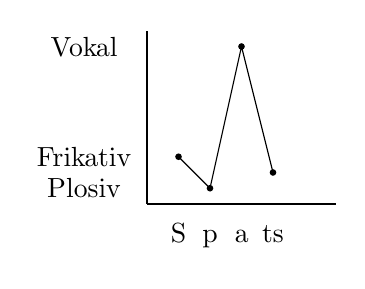
\begin{tikzpicture}[scale=0.4]
\draw[black] (-1,0) -- (5,0) ; % x axis
\draw[black] (-1,0) -- (-1,5.5); % y axis
\node at (-3,0.5) {Plosiv};
\node at (-3,1.5) {Frikativ};
\node at (-3,5) {Vokal};
\draw[black] (0,1.5) -- (1,0.5) -- (2,5) -- (3,1);
\node at (0,-1) {\strut \textipa{S}};
\node at (1,-1) {\strut \textipa{p}};
\node at (2,-1) {\strut \textipa{a}};
\node at (3,-1) {\strut \textipa{\texttoptiebar{ts}}};
\fill (0,1.5) circle [radius=3pt];
\fill (1,0.5) circle [radius=3pt];
\fill (2,5) circle [radius=3pt];
\fill (3,1) circle [radius=3pt];
\end{tikzpicture}
\pause
\hfill
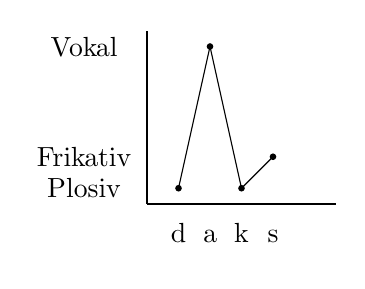
\begin{tikzpicture}[scale=0.4]
\draw[black] (-1,0) -- (5,0) ; % x axis
\draw[black] (-1,0) -- (-1,5.5); % y axis
\node at (-3,0.5) {Plosiv};
\node at (-3,1.5) {Frikativ};
\node at (-3,5) {Vokal};
\draw[black] (0,0.5) -- (1,5) -- (2,0.5) -- (3,1.5);
\node at (0,-1) {\strut \textipa{d}};
\node at (1,-1) {\strut \textipa{a}};
\node at (2,-1) {\strut \textipa{k}};
\node at (3,-1) {\strut \textipa{s}};
\fill (0,0.5) circle [radius=3pt];
\fill (1,5) circle [radius=3pt];
\fill (2,0.5) circle [radius=3pt];
\fill (3,1.5) circle [radius=3pt];
\end{tikzpicture}
\hfill\mbox{}
\vfill
\pause
\hfill
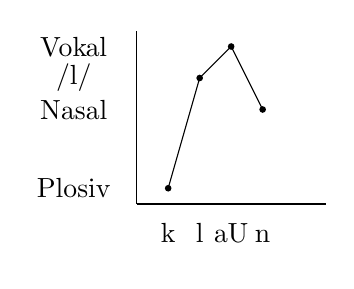
\begin{tikzpicture}[scale=0.4]
\draw[black] (-1,0) -- (5,0) ; % x axis
\draw[black] (-1,0) -- (-1,5.5); % y axis
\node at (-3,0.5) {Plosiv};
\node at (-3,3) {Nasal};
\node at (-3,4) {\textipa{/l/}};
\node at (-3,5) {Vokal};
\draw[black] (0,0.5) -- (1,4) -- (2,5) -- (3,3);
\node at (0,-1) {\strut \textipa{k}};
\node at (1,-1) {\strut \textipa{l}};
\node at (2,-1) {\strut \textipa{\texttoptiebar{aU}}};
\node at (3,-1) {\strut \textipa{n}};
\fill (0,0.5) circle [radius=3pt];
\fill (1,4) circle [radius=3pt];
\fill (2,5) circle [radius=3pt];
\fill (3,3) circle [radius=3pt];
\end{tikzpicture}
\hfill
\pause
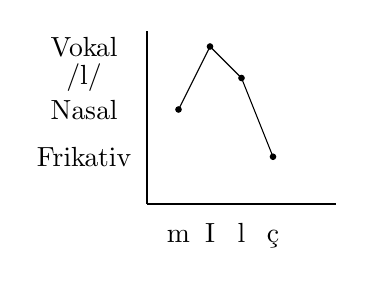
\begin{tikzpicture}[scale=0.4]
\draw[black] (-1,0) -- (5,0) ; % x axis
\draw[black] (-1,0) -- (-1,5.5); % y axis
\node at (-3,1.5) {Frikativ};
\node at (-3,3) {Nasal};
\node at (-3,4) {\textipa{/l/}};
\node at (-3,5) {Vokal};
\draw[black] (0,3) -- (1,5) -- (2,4) -- (3,1.5);
\node at (0,-1) {\strut \textipa{m}};
\node at (1,-1) {\strut \textipa{I}};
\node at (2,-1) {\strut \textipa{l}};
\node at (3,-1) {\strut \textipa{\c{c}}};
\fill (0,3) circle [radius=3pt];
\fill (1,5) circle [radius=3pt];
\fill (2,4) circle [radius=3pt];
\fill (3,1.5) circle [radius=3pt];
\end{tikzpicture}
\hfill\mbox{}
\vfill
\end{frame}


%%%%%%%%%%%%%%%%%%%%%%%%%%%%%%%%%%
\begin{frame}
\frametitle{Übung -- Lösung}

\begin{itemize}
\item Erklären Sie die Ungrammatikalität der folgenden Silben:

\begin{exe}
	\exr{ex:lbat}
	\settowidth\jamwidth{XXXXXXXXXXXXXXXXXXXXXXXXXXXXXXXXXX}
	\begin{xlist}
		\ex[*]{ \textipa{[lbat]}\loesung{2}{\textipa{[l]} vor \textipa{[b]} im Onset} }
		\ex[*]{ \textipa{[blabl]}\loesung{3}{\textipa{[b]} vor \textipa{[l]} in der Koda $+$ Auslautverhärtung} }
		\ex[*]{ \textipa{[m{\textscr}apt]}\loesung{4}{\textipa{[m]} vor \textipa{[\textscr ]} im Onset} }
		\ex[*]{ \textipa{[ki:l\textscr]}\loesung{5}{\textipa{[l]} vor \textipa{[\textscr ]} in der Koda} }
		\ex[*]{ \textipa{[ngang]}\loesung{6}{\textipa{[n]} vor \textipa{[g]} im Onset $+$ reg. velare Nasalassimiliation } \loesung{6}{$+$ g-Tilgung}}
		\ex[*]{ \textipa{[krafm]}\loesung{7}{\textipa{[f]} vor \textipa{[m]} in der Koda} }
		\ex[*]{ \textipa{[elat]}\loesung{8}{2 Silben (2 Nuklei) $+$ Knacklauteinsetzung} }
		\ex[*]{ \textipa{[plaml]}\loesung{9}{\textipa{[m]} vor \textipa{[l]} in der Koda} }
		\ex[*]{ \textipa{[nfatl]}\loesung{10}{\textipa{[n]} vor \textipa{[f]} im Onset $+$ \textipa{[t]} vor \textipa{[l]} in der Koda} }
	\end{xlist}
\end{exe}

\end{itemize}

\end{frame}

